\chapter{Eztabaida.}


Kapitulu honetan, ikerketan zehar garrantzi berezia izan duten gaiak bildu ditugu. Eguzki-sistemaren simulazioetarako eta efemerideen kalkulutarako erabiltzen diren inplementazioen laburpena eman dugu. Ikerketaren lehen urratsean eta gero baztertu genuen planteamenduaren azalpenak eman ditugu. IRK inplementazioaren oinarriak erabakitzeko, aztertutako aukerak deskribatu ditugu. Kepler-en fluxuan oinarritutako aldagai aldaketa, atalen hasieraketan aplikatzeko aukera deskribatu dugu. Zenbakizko integrazioetan, paralelizazioa aplikatzeko zailtasunak azpimarratu ditugu. Azkenik, inplementazioa $N$-gorputzen beste integrazio batzuetan aplika daitekeen aztertu dugu.   


\section{Eguzki-sistemaren integrazio luzeak.}


Gure helburua eguzki-sistemaren epe luzeko eta doitasun handiko inplementazio eraginkorra proposatzea da. Atal honetan, egungo eguzki-sistemaren simulazioetarako erabiltzen diren metodo eta inplementazioen laburpena egingo dugu. 

\subsection*{Inplementazioen garapena.} 

Astronomi arloaren ikerketetan, eguzki-sistemaren eredu errealisten integrazio luzeak konputatzen dituzte. A. Morbidellik \cite{Morbidelli2002}, eguzki-sistemaren zenbakizko integraziotarako inplementazioen azterketa egin zuen: urteak aurrera joan ahala, eguzki-sistemaren ereduak gero eta konplexuagoak bilakatzen dira, eta integrazio tartea handiago da. Garai hauek bereizten ditu:
\begin{enumerate}

\item Garai klasikoa.

$90$. hamarkada artekoa, urrats luzera aldakorreko integratzaileak erabiltzen dira: Runge-Kutta (Dormand et al. $1987$), Bulirsch and Stoer ($1966$), Radau (Everharht, $1985$), eta Störmer ($1990$). Garai honetan, integrazio tarteak ($10^4-10^6$) urte artekoak dira.  

\item Garai sinplektikoa.

Wisdom eta Holman-en \cite[1991]{Sussman1992} lanarekin, eguzki-sistemaren azterketarako integratzaile sinpletikoen erabilera zabaldu zen. Garai honetan, ($10^8-10^9$) urte arteko eguzki-sistemaren integrazioak egin ziren.  

\item Garai estatistikoa.

Planeten, eta asteroideen edota meteoritoen moduko gorputz txikien  arteko kolisiotik gertuko egoerak kalkulatzen dituzten algoritmoak garatu ziren. Inplementazio berri hauetan, milaka gorputzen integrazio azkarra egin daiteke. Asteroide eta meteoritoen orbiten distribuzio azterketa estatistikoak egin zituzten.

\item Planeten sorrera garaiko azterketak.

Garai honetan, eguzki-sistemaren sorrerari buruzko simulazioak nagusi dira; masa handiko gorputzen arteko kolisiotik gertuko egoerak gertatzen diren problemak konputatzen dira. 
 
\end{enumerate}

Astronomi arloko eguzki-sistemaren integrazioetarako, nagusiki bi integratzaile famili bereiz daitezke \cite{Ito2007}; metodo simetrikoak eta sinplektikoak. Bestalde, integrazio metodo orokorrak, efemerideen konputazioetarako aplikatzen dira. 
\begin{enumerate}
\item Metodo simetrikoak.

Metodo simetrikoen artean nagusiena, 4 ordenako \emph{Hermite}  integratzailea \cite{Aarseth2008} dugu.
Urrats luzera tamaina aldakorreko integratzaile da.  \emph{Hermite} integratzailea konputazionalki garestia da eta gorputz kopuru handia duten eta kolisiotik gertuko egoerak maiz gertatzen diren problemetan aplikatzen da; esate baterako, eguzki-sistemaren sorreraren azterketarako.  

\item Metodo sinplektikoak.

Egungo eguzki-sistemaren epe luzeko integrazioetarako, integratzaile sinplektikoak nagusitu dira. 

\item Metodo orokorrak.

Efemerideen doitasun altuko integrazioetarako, metodo orokorrak erabiltzen dituzte: \emph{Multistep Adams} metodoa (NASA), \emph{Adams-Cowel} metodoa (IMCCE, Paris Observatory) eta \emph{Radau} metodoa (IAA, St. Petersburg). 

\end{enumerate}


\subsection*{Metodo sinplektikoak.}

Wisdom eta Holman-en \cite[1991]{Sussman1992} eguzki-sistemaren epe luzeko simulazioetarako integratzaile  sinplektikoak (\emph{WH}) arrakasta izan zuen. Eguzki-sistema, mugimendu perturbatua duen sistema dinamikoa da eta ezaugarri honi egokitutako integratzaile eraginkorra garatu zuten. Jacobi koordenatuak  aplikatuz, N-gorputzen problemaren Hamiltondarra, bi zatitan banatu zuten,
\begin{equation*}
H(q,p)=H_K(p)+H_I(q) \ \ \ , \ \ H_K\gg H_I,
\end{equation*}
non $H_K$, Hamiltondarraren alde Kepleriarra (planeten eguzkiarekiko mugimendu Kleperiarra) eta $H_I$, Hamiltondarraren perturbazioa (planeten arteko interakzioak) diren. Integrazioaren urrats bakoitzean, Hamiltondar bakoitzaren soluzioa tartekatuz, problema osoaren soluzioa lortzen da.  

%inplementazio askoren aurrekaria kontsideratu bada ere, bere aplikagarritasuna mugatua da. 
\emph{WH} inplementazioaren erabilgarritasuna mugatua da. Batetik, izar anitzeko planeten sistemak edo planeta-ilargiak sistemak integratzeko ez da egokia. Bestetik, \emph{WH} metodo sinplektikoa denez, urrats luzera finkoa aplikatu behar da eta hau, gorputzen arteko kolisiotik gertuko egoerak dituzten problemak modu eraginkorrean integratzeko eragozpen bat da. Arazo hauek gainditzeko, hurrengo urteetan  algoritmo honen aldaerak proposatu dira. 

Levinson eta Duncan-ek \cite[1994]{Levison1994}, \emph{WH} inplementazioa, integratzaile ez sinplektiko batekin konbinatu zuten, kolisiotik gertuko egoeren kalkulua hobetzeko. \emph{SWIFT} paketean, \emph{RMVS3} izeneko integratzailea inplementatu zuten. Duncan, Levinson eta Lee-k \cite[1998]{Duncan1998}, koordenatu heliozentrikoak erabiliz, Hamiltondarra beste modu honetan banatu zuten,  
\begin{equation*}
H(q,p)=H_K(p)+(H_C(p)+H_I(q))
\end{equation*}
eta kolisiotik gertuko egoerei, urrats luzera txikituz aurre egin zioten. Inplementazio honek, \emph{SYMBA} izena du. Chambers \cite{Chambers1999}, koordenatu heliozentrikoetan oinarritu zen eta kolisiotik gertuko egoerak gertatzen diren uneetan, \emph{WH} inplementazioa, beste integrazio metodo batekin (Bulirsch-Stoer metodoa) konbinatu zuen. Inplementazio honek, \emph{MERCURY} izena du. %Levinson eta Duncan-ek ($2000$), aurreko inplementazioaren arazo batzuk konponduz, \emph{Modified SYMBA} izeneko garapen berria burutu zuten.
Kvaerno eta Leimkuhler \cite{Kvaerno2000} eta beste autore batzuk ere, antzeko ideiak landu dituzte.

%Eszentrikotasun handiko orbita duten sistementzako hainbat “erregularizazio sinplektiko integratzaileak“ aztertu dira:
%Levison and Duncan (1994). “RMVS”: Regularized mixed variable sympletic integrator”, Mikkola (1997), Fukushima (2001), Beus(2003).
%Erregularizazioa aplikatzen dituzte metodo simpletiko ezbedinen “review” honakoa dugu: “Rauch
%and Holman (1999). Dynamical chaos in the Wisdom-Holman integrator”.

Wisdom eta Holmanek proposatutako Hamiltondarraren banaketa, (\ref{eq:stverlet})~\emph{Leapfrog} metodoaren bidez integratzen da eta beraz, $p=2$ ordenako da. Ordena altuagoko ($p>2$) metodo sinplektikoak definitzeko, koefiziente negatiboak erabili behar zirela uste zen \cite{Yoshida1993,Laskar2001} eta modu honetan definitutako metodoak, ez dira \emph{Leapfrog} metodoa baino eraginkorragoak.

McLachlan-ek \cite[1995]{McLachlan1995} eta Laskar-ek  \cite[2001]{Laskar2001} koefiziente negatiboen arazoa gainditu zuten eta koefiziente positiboekin definitutako ordena altuko splitting eskemak aurkitu zituzten. Berriki, Blanes-ek \cite[2012]{Blanes2013} ordena altuko splitting eskema  eraginkorrak aurkitu ditu. 

Hernandez eta Bertschinger-ek \cite[2015]{Hernandez2015} N-gorputzen problema grabitazionala eta kolisiotik gertuko egoerak integratzeko, $2$ ordenako metodo sinplektiko berri bat proposatu dute. Hernandez eta Bertschinger-ek \cite{Hernandez2015} koordenatu cartesiarretan oinarrituz, $N$-gorputzen problema $2$-gorputzen azpiproblemetan banatzen dute.


\subsection*{Konposizio eta splitting metodoak.}


Konposizio metodoak, era honetako Hamiltondar sistemak integratzeko aplika daitezke,
\begin{equation*}
H(q,p)=T(p)+Uq).
\end{equation*}

Konposizio metodoa, eguzki-sistemaren eredu grabitazionalari aplikatzerakoan oso eraginkorra da, baina eredu konplexuagoetarako bere abantaila galtzen du. Batetik, gorputzen kopurua handitzen bada bere eraginkortasuna gutxitzen da eta bestetik, beste indar ez grabitazionalak (erlatibitate efektua,\dots) ezin daitezke aplikatu.

Splitting metodoak, era honetako Hamiltondar sistemak integratzeko aplika daitezke, 
\begin{equation}
\label{eq:Hban}
H=H_A+\epsilon H_B,
\end{equation}
non $H_A$ eta $H_B$ independenteki integratu daitezkeen. 

Eguzki-sistemaren eredu errealistetan, hainbat indar ez grabitazional modu honetan gehitzeko, zailtasunak izan ditzakegu.
Laskar-ek \cite[2011]{Laskar2011}, epe luzeko zenbakizko integraziorako,  eguzkiaren erlatibitate efektua ($1/c^2$ ordenakoa)  kontsideratu zuen, Saha eta Tremain-ek \cite{Saha1994} finkatutako teknika aplikatuz. Teknika honen bidez, Hamiltondar banagarriei egokitzen zaien erlatibitate efektuaren espresioa lortzen da eta gainera modu eraginkorrean kalkulatzen da. Baina splitting metodoetan, beste planeten erlatibitate efektuak ezin daitezke erabili. Adibidez, bi planeta handienen (Jupiter eta Saturno) erlatibitate efektua ere kontutan hartuko balira, ekuazioak ez dira gehiegi konplikatzen eta integrazio hobea lor daiteke, errorea txikituz. 
 
Eguzki-sistemaren integrazioetarako, (\ref{eq:Hban}) Hamiltondarraren banaketa, Jacobi koordenatuak edo heliozentrikoak aplikatuz lortzen da.
Koordenatu cartesiarrak, ezin daitezke erabili.

IRK metodoekin lan egiteko ordea, ez daukagu halako mugarik. Ekuazio diferentzial orokorrei aplika dakizkienez, askatasun osoa dugu behar diren ekuazioak erabiltzeko eta interesatzen zaigun koordenatu sistema aplikatzeko.  


\section{Eredu deskonposaketa.}


IRK metodoen inplementazioen azterketaren hasieran, eredu deskonposaketan oinarritutako ideia ikertu dugu. Atal honen bukaeran emango ditugun arrazoiengatik, beste bide batzuk ikertzea zuzenago dela ikusi dugu eta planteamendu hau alde batera utzi dugu. Dena den, planteamendu honen laburpen bat emango dugu eta inplementazio bide honetan sortutako hainbat ideia interesgarri jasoko ditugu.

Eguzki-sistemaren eredua bi zatitan bana daiteke: problema sinplea (konputazionalki merkea) eta problema konplexua (konputazionalki garestia). Newton sinplifikatuaren iterazio berezi bat aplikatu dugu, problema konplexuaren balioztapen kopurua txikitzeko eta era honetan, inplementazio eraginkorra lortzeko. Newton sinplifikatuaren iterazio berezi honetan, ekuazio-sistema lineala LU deskonposaketaren bidez askatu beharrean, puntu-finkoaren bidez ebatziko dugu.


\subsection*{Inplementazioa.}
Eguzki-sistema, perturbatutako mugimendu Kepleriar gisa har daiteke,  
\begin{align}
\label{eq:fkg}
 f(y)=  k(y) + \epsilon \ g (y), \ \ g\ll k.   
\end{align}
 
$k(y)$ sistema dinamikoaren alde sinplifikatua da eta konputazio kostu txikia du. $g(y)$, ordea, sistemaren alde konplexua da eta konputazio kostu handia du. (\ref{eq:fkg}) ekuazio diferentzialak IRK metodoen bidez integratzeko, atalen ekuazio-sistema inplizitua ebatzi behar da: 
\begin{equation*}
Y_i=y_n+h\ \ \sum^s_{j=1}{a_{ij} \ f({Y_j}) }. 
\end{equation*} 
%
Ekuazio inplizituaren sistema hau, honako iterazioaren bidez ebaztea proposatuko dugu:
\begin{align}
\begin{split}
&k=1,2,\dots \\
&Y_i^{[k]}=y_n+h\ \ \sum^s_{j=1}{a_{ij}(\ k({Y_j}^{[k]})+g({Y_j}^{[k-1]})) }
\end{split}
\end{align}

Iterazio hau aplikatzea, Jacobiarraren hurbilpentzat, $J_i=\partial k/ \partial y (Y_i), \ i=1,\dots,s$ hartzen duen Newton sinplifikatua aplikatzearen baliokidea da. \ref{alg:metalg} algoritmoan, iterazioa aplikatzeko zehaztasun gehiago emango ditugu,
 
\begin{algorithm}[H]
 \For{$n\leftarrow 1$ \KwTo $endstep$}{
  \BlankLine
  \text{Hasieraketa}\ $Y^{[0]}_i, W^{[0]}_i$\;
  k=1\;
  \text{Askatu} \ ${Y_i}^{[k]}=y_n+h\  \sum^s_{j=1}{a_{ij}\ k({Y_j}^{[k]})+W^{[k-1]}_i\ \ \ }$\;
  \BlankLine
  \While{(\text{konbergentzia ez lortu})}{
     \BlankLine
     k++\;
     $W^{[k-1]}_i= h\ \sum^s_{j=1}{a_{ij}\ g({Y_j}^{[k-1]})}$\; 
     \text{Askatu} \ ${Y_i}^{[k]}=y_n+h\  \sum^s_{j=1}{a_{ij}\ k({Y_j}^{[k]})+W^{[k-1]}_i\ \ \ }$\;
     \BlankLine
  }  
  $y_{n+1}=y_n+h\ \sum^s_{j=1}{b_{i}\ f({Y_j}^{[k]}) \ }$\;
  \BlankLine
 }
 \caption{Meta-algoritmoa}
 \label{alg:metalg}
\end{algorithm}

%Meta-algoritmoaren barne ekuazio-sistema askatzeko, 
Urrats bakoitzean, hainbat aldiz $k=2,3,\dots$ balioentzat ekuazio-sistema inplizitua askatu behar da eta horretarako, 
metodo egokiena aplikatzeko askatasuna dugu. Pentsa liteke,  problema zurruna ez bada puntu-finkoaren bidez askatzea eta problema zurruna bada, berriz,  Newton sinplifikatuaren iterazioaren bidez.

Barne ekuazio-sistema,
\begin{equation*}
 Y_i^{[k]}=y_n+h\  \sum^s_{j=1}{a_{ij}\ k({Y_j}^{[k]})+W^{[k-1]}_i},
\end{equation*}
puntu-finkoaren iterazioaren bidez askatzeko, \ref{alg:bpf}~algoritmoaren barne-iterazioa era honetan aplikatuko dugu: 

\begin{algorithm}[H]
 \BlankLine
  $l=0$\;
  $Y_{i}^{[k,0]}=Y_{i}^{[k-1]}$\;
  \While{ (\text{konbergentzia ez lortu})}
  {
   \BlankLine
   $l=l+1$\;  
   \BlankLine
   $K_{i}^{[k,l]}=k(Y_{i}^{[k,l-1]})$\;
   $Y_{i}^{[k,l]}=y_{n} + h \sum\limits_{j=1}^{s} \ a_{ij} \ K_{j}^{[k,l]}  +  W_{i}^{[k-1]} $\;
  }
 \caption{Barne-iterazioa: puntu-finkoaren iterazioa}
 \label{alg:bpf}
\end{algorithm}


\subsection*{Orokorpena.}

\subsubsection*{Eredu konplexuak.}
Aurreko atalean, maila bakarreko ereduen deskonposaketa aztertu dugu. Ideia orokortuz, eredu deskonposaketa maila ezberdinetan aplika daiteke.  $\dot{y} =f(y)$ problema emanik, 
\begin{align*}
&\mbox{1. maila} \ \
\left \{ \begin{array}{c}
  \mbox{Eredu osoa.   } f(y) \\[.25cm]
  \mbox{Eredu sinplea.    } \tilde{f}(y)  \\
\end{array} \right.
\ \Rightarrow \ \
f =\tilde{f}+(f-\tilde{f})  
\end{align*}

\begin{align*}
&\mbox{2. maila} \ \
\left \{ \begin{array}{c}
  \mbox{Eredu osoa.   }\tilde{f}(y) \\[.25cm]
  \mbox{Eredu sinplea.    }\tilde{\tilde{f}}(y)  \\
\end{array} \right.
\ \Rightarrow \ \
\tilde{f} =\tilde{\tilde{f}}+({\tilde{f}}-\tilde{\tilde{f}})\\
&\dots  
\end{align*}

\paragraph*{Adibidea.}
Eguzki-sistemaren eredu konplexuaren ekuazio-sisteman, alde Kepleriarra eta perturbazio maila ezberdinak bereiz daitezke. Algoritmoa, deskonposaketaren maila bakoitzari modu errekurtsiboan aplika daiteke. Demagun, eguzki-sistemaren problemaren ekuazio diferentzial hauek ditugula,
\begin{equation*}
\dot{y}=f(y), \ f(y)=k(y)+g(y)+r(y),
\end{equation*}
non
\begin{align*}
&k(y): \ \text{kepleriarra.}\\
&g(y): \ \text{planeten arteko grabitazio interakzioak.}\\
&r(y): \ \text{planeten eguzkiarekiko erlatibitate efektua.}
\end{align*}

Meta-algoritmoa modu honetan aplika daiteke,
\begin{align*}
&\mbox{1. maila}\\ 
&Y_i=y_n+h \ \sum^s_{j=1}{a_{ij} \ f(Y_j)}.\\
&\mbox{2. maila}, \ k=1,2,\dots\\
&Y_i^{[k]}=y_n+h\  \sum^s_{j=1}{a_{ij} \ k({Y_j}^{[k]})}+ \delta_1^{[k-1]},\\
& \text{non} \ \ \delta_1^{[k-1]}= h\  \sum^s_{j=1}{a_{ij} (g({Y_j}^{[k-1]})+r({Y_j}^{[k-1]}))}. \\
&\mbox{3. maila}, , \ l=1,2,\dots\\
&Y_i^{[k,l]}=y_n+h\ \ \sum^s_{j=1}{a_{ij} \left(k({Y_j}^{[k,l]})+g({Y_j}^{[k-1,l]})\right)}+\delta_2^{[l-1]}, \\
& \text{non} \ \ \delta_2^{[l-1]}= h \ \sum^s_{j=1}{a_{ij} \ r({Y_j}^{[k-1,l-1]})}.
\end{align*}


\subsubsection*{Problema independenteak.}

Batzuetan, problemaren eredu sinplifikatua, azpiproblema independentetan bana daiteke,
\begin{align*}
f\left ( \begin{array}{c}
   y_1 \\
   y_2 \\
\end{array} \right)=
\left ( \begin{array}{c}
   k_1(y_1) \\
   k_2(y_2) \\
\end{array} \right)+
\left ( \begin{array}{c}
   g_1(y_1,y_2) \\
   g_2(y_1,y_2) \\
\end{array} \right).
\end{align*}
%
Azpiproblema bakoitzari dagokion barne-iterazioak independenteak dira eta paraleloan kalkula daitezke. Eguzki-sistema eredu grabitazionala, azaldutakoaren adibide argia da; planeta bakoitzaren $k_i(y)$ eguzkiarekiko interakzioa, azpiproblema independentea da. Zenbakizko esperimentuetarako aukera eraginkorrena, eredu sinplifikatua bi azpiproblemetan banatzea dela konprobatu dugu: alde batetik, barne-planeten eredu sinplifikatuak osatutako azpiproblema eta beste aldetik, kanpo-planeten eredu sinplifikatua osatutakoa.    

\subsubsection*{Tolerantzia aldakorra.}

Kanpo eta barne-iterazioetarako geratze irizpide berdinak definitu ditugu. Kanpo-iterazioetarako, tolerantzia finkoa erabili dugu eta barne-iterazioetarako, ordea, tolerantzia aldakorra. Tolerantzia aldakorra, kanpo-iterazio (konputazionalki garestia) bakoitzarentzat, barne-iterazio (konputazionalki merkea) kopuru nahikoak eta beharrezkoak eman daitezen, definitu dugu.     
 

\subsection*{Eragozpenak.}
Esan dugunez, planteamendu honetan Newton sinplifikatua aplikatu dugu eta ekuazio-sistema lineala LU deskonposaketaren bidez askatu beharrean, puntu-finkoaren iterazioaren bidez askatu dugu. Planteamendu honi IRK-Newton sinplifikatuaren inplementazio estandarrarekiko, hiru desabantaila aurkitu dizkiogu: 
\begin{enumerate}
\item Barne kalkuluen doitasuna. 

Planteamendu honen barne-iterazioak, inplementazioaren oinarrizko doitasunean kalkulatu behar dira.
IRK-Newton sinplifikatuaren inplementazioaren eragiketa konplexuenak, doitasun txikiagoan kalkula daitezke \cite{Baboulin20092526}. 

\item Jacobiarraren balioztapena.

Planteamendu honetan, Jacobiarra iterazio bakoitzean aldatzen denez, iterazio guztietan balioztatu behar da.
IRK-Newton sinplifikatu estandarrean, Jacobiarra urrats bakoitzean behin bakarrik kalkulatu behar da. 

\item Ereduen deskonposaketa.\\
Ereduen deskonposaketak, nolabaiteko konplexutasuna gehitzen du. Hiru eredu ezberdin bereizi behar ditugu: eredu osoa $f(y)$, eredu sinplifikatua $\tilde{f}(y)$ eta perturbazioa  $g=f(y)-\tilde{f}(y)$. 
\end{enumerate}

\section{IRK inplementazioaren oinarriak.}


\emph{IRK} inplementazioan, ekuazio-sistema iterazio metodo bat aplikatuz askatu behar da. Funtsezkoa da, iterazioaren atalen hasieraketa eta geratze irizpide sendoak aplikatzea. Laburki, gure lanean aztertutako aukera ezberdinak deskribatuko ditugu.  

\subsection*{Atalen hasieraketa.}

Iterazio metodoetan  atalen hasieraketa kalkulatzeko teknika ezberdinak ikertu ditugu. 
\begin{enumerate}
\item Metodo esplizituak.

Atalen hasieraketa metodo esplizitu bat aplikatuz lor daiteke. Hurbilpen merkea lortze aldera, ordena txikiko metodoak aplikatu ditugu: 
Euler  $\mathcal{O}(h)$ eta Euler hobetuaren $\mathcal{O}(h^2)$ metodoa. Atalen hasieraketa metodo hauetan, ekuazio diferentzialaren balioztapena beharrezkoa da eta era honetan aplikatu ditugu:
\begin{align*}
&\text{Euler}:\\
& \quad Y_i=Y_{i-1}+h (c_i-c_{i-1}) f(Y_{i-1}).\\
&\text{Euler hobetua}: \\
& \quad Y_i=Y_{i-1}+h (c_i-c_{i-1}) f(k_i),\\
& \quad \text{non} \ k_i=Y_{i-1}+\frac{h}{2} (c_i-c_{i-1}) f(Y_{i-1}).
\end{align*} 


\item Kepler-en fluxua.

Eguzki-sistema, perturbatutako sistema Kepleriarra denez, atalak Kepler fluxuaren bidez hasieratu daitezke. Kepler fluxuaren funtzioak, $y(t_n)$ une bateko kokapen eta abiadurak emanik, $\Delta t_n$ denbora igarotakoan kokapen eta abiadura zehatzak itzultzen ditu,
\begin{equation*}
\text{Keplerflow}(\Delta t_n, y(t_n)) \rightarrow y(t_n+\Delta t_n).
\end{equation*}

Beraz, $y_n$ egoeratik abiatuta, atal bakoitzari dagokion hasieraketa,
\begin{equation*}
Y_{n,i}^{[0]}=y(t_n+hc_i), \ i=1,\dots,s,
\end{equation*}
Kepler fluxua $\Delta t_n=hc_i$ denbora aurrera eginez lortuko dugu.  

\item Interpolazio polinomioak.

Aurreko urratseko ataletako informazioa erabiliz, urrats berriaren atalen hasieraketa lortzen dugu. Problema ez-zurrunetarako interesgarria da. Era honetako hasieraketa merkea da, ez baita funtzio balioztapen berririk egiten. Era honetan aplikatzen da,
\begin{equation*}
Y_{n,i}^{[0]}=y_n+h \sum_{j=1}^{s} \lambda_{ij} \ f(Y_{n-1,j}),
\end{equation*}
non $\lambda_{ij}$ aurre-kalkulatutako interpolazio koefizienteak diren. Interpolazio metodo estandarrarekin, urrutien dagoen ataletarako hasieraketa txarra lortzen da eta atal askotako metodoentzat, arazo hau, eragozpen handia izan daiteke. 


Bide honetatik, teknika aurreratuagoak ere aztertu ditugu (maila txikiko polinomioen bidezko hasieraketak,\dots). Era berean, B-Serieak izeneko teknikan \cite{Chartier2010} oinarrituz, interpolazio estandarra \cite{Laburta1998} hobetzeko saiakera egin dugu baina ez dugu arrakastarik izan.  

\end{enumerate}

Problema ez-zurrunetarako, interpolazio polinomioen bidezko hasieraketa ona eta merkea lortzen da. Problema zurrunetarako, ordea, atalak aurreko urratseko soluzioarekin hasieratuko ditugu,
\begin{align*}
Y_{n,i}^{[0]}=y_n, \ i=1,\dots,s.  
\end{align*}
    

\subsection*{Geratze irizpidea.}

Iterazio metodo bat aplikatzeko, geratze irizpide sendoa finkatzea funtsezkoa da.  Iterazioak, biribiltze errorearen eragina azaltzen denean geratu behar dira. Batetik, iterazioak beranduegi geratzen baditugu, alferrikako iterazioak emango ditugu, eraginkortasunaren kalterako. Bestetik, iterazioak goizegi geratzen baditugu, biribiltze errorea handitu edota trunkatze errorea eragin dezake.  

Geratze irizpide estandarrak aplikatzerakoan, hainbat arazo aurkitu ditugu eta ondorioz, geratze irizpide berri bat definitzeko beharra ikusi dugu. Geratze irizpide berria definitzeko, aukera ezberdinak aztertu ditugu eta eskuartean ibili ditugun bertsio nagusienak azalduko ditugu.      

\subsubsection*{Norma.}
Iterazio bakoitzaren hobekuntza ($\Delta^{[k]}$) neurtzeko, norma ezberdinak aplikatu daitezke. Honakoa da,  Hairer-ek bere IRK inplementazioaren geratze irizpidean aplikatzen duen norma,
\begin{equation*}
\Delta^{[k]}= \max_{i=1,\dots,s} \|Y_i^{[k]}-Y_i^{[k-1]}\|_{\infty}.
\end{equation*}

Norma hau zalantzan jarri dugu eta iterazioaren hobekuntza hobeto neurtzen duen norma finkatzen saiatu gara. Honako aukerak aztertu ditugu:
\begin{enumerate}
\item Lehen bertsioa.

Diferentziak, modu erlatiboan neurtzeko beharrak bultzatuta, norma era honetan definitu dugu,
\begin{align*}
\Delta=\max_{1 \leqslant j \leqslant d} \frac{\max_{1 \leqslant i \leqslant s} |\Delta Y_i^j|}
                                                {(\max_{1 \leqslant i \leqslant s}|Y_i^j|)+\delta},
\end{align*}
non $\delta \approx 10^{-20}$, zatitzailea zero ez izateko finkatzen dugun balio txikia  eta $y=(y^1,\dots,y^d)$ den.

\item Bigarren bertsioa.

Kokapenen ($Q_i \in \mathbb{R}^d$) eta abiaduren ($V_i \in \mathbb{R}^d$) izaera ezberdina dela jabetuta, norman bi kontzeptu hauek banatu ditugu. $Y=Y^{[k]}, \ \text{eta} \ \tilde Y=Y^{[k-1]}$ notazioa finkatuta,
\begin{align*}
 & \Delta =\\
 & max\left({\  {\max_{1\le j\le d} \frac{{\max_{1\le i\le s} {\left\|Q^{j}_i-{\tilde{Q}}^{j}_i\right\|}^2\ }}{{\max_{1\le i\le s} {\left\|Q^{j}_i\right\|}^2\ }}\ }\ },\ {\max_{1\le j\le d} \frac{{\max_{1\le i\le s} {\left\|V^{j}_i-{\tilde{V}}^{j}_i\right\|}^2\ }}{{\max_{1\le i\le s} {\left\|V^{j}_i\right\|}^2\ }}\ }\right),
\end{align*}
non, 
\begin{align*}
Y=\left( \begin{array}{cccccc}
Q^{1}_1 & \dots  & Q^{d}_1 & V^{1}_1 & \dots  & V^{d}_1 \\ 
Q^{1}_2 & \dots  & Q^{d}_2 & V^{1}_2 & \dots  & V^{d}_2 \\ 
\vdots  & \ddots  & \vdots  & \vdots  & \ddots  & \vdots  \\ 
Q^{1}_s & \dots  & Q^{d}_s & V^{1}_s & \dots  & V^{d}_s \end{array}
\right)\ \  
\tilde Y=\left( \begin{array}{cccccc}
\tilde Q^{1}_1 & \dots  & \tilde Q^{d}_1 & \tilde V^{1}_1 & \dots  & \tilde V^{d}_1 \\ 
\tilde Q^{1}_2 & \dots  & \tilde Q^{d}_2 & \tilde V^{1}_2 & \dots  & \tilde V^{d}_2 \\ 
\vdots  & \ddots  & \vdots  & \vdots  & \ddots  & \vdots  \\ 
\tilde Q^{1}_s & \dots  & \tilde Q^{d}_s & \tilde V^{1}_s & \dots  & \tilde V^{d}_s \end{array}
\right). 
\end{align*}

\item Hirugarren bertsioa.

Iterazioaren hobekuntza, norma jakin bat aplikatuz zenbaki eskalar bakarrarekin neurtu beharrean,
\begin{equation}
\label{eq:DD3}
\Delta^{[k]}=|Y^{[k]}-Y^{[k-1]}| \in \mathbb{R}^{sd}
\end{equation}
matrizea erabiliko dugu. Modu honetan, geratze irizpidea normaren independentea izango da eta gainera, geratze irizpide segurua eraikitzeko aukera emango digu.

\end{enumerate} 


\subsubsection*{Geratze irizpidea.}

Geratze irizpidearen abiapuntua Hairer-en geratze irizpidea izan da,
\begin{equation*}
\Delta ^{[k]}=0 \ \text{edo} \ \Delta^{[k]} \geqslant \Delta^{[k-1]}.
\end{equation*}

Geratze irizpide hau hobetzeko proposamen batzuk garatu ditugu,
\begin{enumerate}
\item Lehen bertsioa.

Hairer-ek definitutako geratze irizpidea, batzuetan goizegi geratzen da eta ziurtasuna handitu beharra dago.  Horregatik, geratze irizpidean, $k-2.$ iterazioaren informazioa erabiltzea aztertu dugu, 
\begin{align*}
(\Delta^{[k]} = 0) \ \text{edo} \ ( \Delta^{[k]}\geqslant \Delta^{[k-1]} \ \ \text{eta} \ \ \Delta^{[k]}\geqslant 0.81*\Delta^{[k-2]}).
\end{align*}

\item Bigarren bertsioa.

Bertsio honetan, $k-3.$ iterazioaren informazioa ere erabiliz saiakera berria proposatu dugu:
\begin{align*}
\left(\Delta^{[k]} \leqslant tol \right) \ \text{edo} \ \left( zat^{[k]} \geqslant koef*\max(zat^{[k-1]},zat^{[k-2]}) \right),
\end{align*}
non $zat^{[k]}={\Delta^{[k]}}/{\Delta^{[k-1]}}, \ tol\approx10^{-16}$ eta $koef=10$ den.

\item Hirugarren bertsioa.
\begin{align*}
\left(\Delta^{[k]} \leqslant tol\right) \ \text{edo} \ \left(\frac{zat^2}{(1-zat)} \Delta^{[k-1]} \leqslant tol\right) \ \text{edo} \ \left(\frac{zat}{(1-zat)}\Delta^{[k-2]} \leqslant tol\right),
\end{align*}
non $zat=\max(zat^{[k-1]},zat^{[k-2]})$, $tol\approx10^{-16}$ den.

Geratze irizpide honetan, iteraziotik irteten denean, $z\geqslant1$ betetzen bada,
\begin{align*}
&(1). \ \Delta {[k]} > c \ tol \rightarrow \text{konbergentzia arazoak (exekuzioa geratu)},\\
&(2). \ \Delta {[k]} \leqslant c \ tol \rightarrow \text{birbiltze errorea (exekuzioa jarraitu)},
\end{align*}   
non $c\approx 10^{4}$ konbergentzia koefizientea den. 

\item Laugarren bertsioa.

Azkenik, honakoa proposatu dugu: (\ref{eq:DD3}) $\Delta ^{[k]} \in \mathbb{R}^{sd}$ izanik, iterazioak  $k=1,2,\ldots$ jarraitzea , $ \Delta^{[k]} =0$ bete arte edo honako baldintza bi iterazio jarraietan betetzen den artean,
\begin{equation*}
\forall j \in \{1,\ldots,s d\},  \quad
\min \left(\{|\Delta_j^{[1]}|,\cdots ,|\Delta_j^{[k-1]}|\} \ /\{0\} \right) \leqslant |\Delta_j^{[k]}|.
\end{equation*}

Geratze irizpide honetan, iterazioak bukatu ondoren $\exists j,  \ \Delta_{j}^{[K]} \neq 0$ betetzen bada, orduan urratsa onargarria den ala ez erabaki behar dugu. 


\end{enumerate}

 
\section{Doitasun altuko konputazioak.}


Konputazio zientzian, nagusiki doitasun bikoitzeko aritmetika (64-bit) aplikatzen da baina eguzki-sistemaren epe luzeko integraziorako, doitasun bikoitza ez da nahikoa. Jarraian, zenbakizko integrazio hauetan \cite{Laskar2015}, doitasuna hobetzeko bi bide azalduko ditugu. 

\subsection*{$80$-biteko doitasuna.}

Egungo \emph{IEEE-754} ($2008$) estandarrak , koma-higikorreko hiru formatu definitzen ditu: arrunta ($32$-bit), bikoitza ($64$-bit) eta laukoitza ($128$-bit).  \emph{IEEE-754} ($1985$) estandar zaharrak , $80$-biteko formatuaren (\emph{double-extended} izenekoa) inplementazioa aholkatzen zuen \cite{Overton2001} baina egungo estandarretik kanpo utzi dute. $80$-biteko doitasunak, $19$ zifra hamartarreko doitasuna eskaintzen du.   

C lengoaiaren \emph{long double} datu motak, $80$-biteko koma-higikorreko aritmetika sustatzen du.  \emph{IA-32} koma-higikorreko eragiketa multzoak \cite{Muller2009}, $80$-biteko zenbaki formatua onartzen du; $64$-biteko mantisa eta $15$-biteko esponentearekin. \emph{IA-64} eragiketa multzoak, $82$-biteko formatu onartzen du; $64$-biteko mantisa eta $17$-biteko esponentearekin. 

Intel $x86$  prozesadoreek, esaterako Intel Xeon Phi \cite{IntelXeon2013} doitasun arrunta eta bikoitza hardwarez inplementatzen dute; laukoitza, softwarez; eta $80$-biteko doitasuna ere hardwarez.

Laskar-ek \cite{Laskar2011,Laskar2015}, eguzki-sistemaren epe luzeko zenbakizko integraziorako, batura konpentsatua eta $80$-biteko koma-higikorra erabili zituen. Integratzaile sinplektikoa C lengoaian berridatzi zuen, Intel-en $80$-biteko aritmetika erabili ahal izateko.
Era berean, efemerideen kalkuluetarako antzekoa gertatu da: EPM \cite{Pitjeva2014} (aplikazioa berridatzi zuten) eta INPOP \cite{Fienga2008} efemerideen kalkulutarako, $80$-biteko aritmetika erabiltzen dute.

Honek, astronomoentzat, soluzioen doitasuna hobetzeak duen garrantzia erakusten digu. $128$-biteko aritmetikaren inplementazioa software bidezkoa da eta erabiltzeko garestiegia. $80$-biteko aritmetikarekin eta batura konpentsatuarekin, zifra hamartar batzuk irabazten dituzte, konputazio kostu nahiko txikiarekin. 
%baina inplementazioen eraginkortasunarekiko eragin txikiarekin.

%Gure IRK metodoen inplementazioak, doitasun bikoitzarekin garatu ditugu. 
$80$-biteko doitasuna abantailak ditu baina doitasun hau erabiltzeak, hainbat errezelo sortzen ditu. 
 \emph{IEEE-754} estandarretik kanpo dago eta hardwarearen menpekoa da. Gainera, Laskar-en \cite{Laskar2011} zenbakizko integrazioen arabera, konputazioak $x2$ garestitu zaizkio. 


\subsection*{Doitasun nahasia.}


Azken urteetan, beharrezko doitasuna lortzeko, koma-higikorreko doitasun ezberdinak nahasteko joera dago. 

Doitasun arrunteko aritmetikak ($32$-bit), doitasun bikoitzarekiko ($64$-bit) $x2$ aldeko eraginkortasun erratioa  du \cite{Dongarra2017}. Aplikazio batzuetarako, doitasun arrunteko doitasuna nahikoa da eta beste batzuetarako, konputazioaren funtsa doitasun arruntean egin daiteke eta galdutako digituak modu merkean berreskuratu.

Doitasun laukoitza ($128$-bit), software bidez modu errazean  inplementatu daiteke. Doitasun laukoitzeko zenbaki bat, doitasun bikoitzeko bi zenbakiren bidez adieraz daiteke. Ideia da, konputazioa doitasun bikoitzean egitea eta doitasun laukoitzean integrazioaren kalkulu zehatz batzuk egitea. Zenbakizko integrazioetarako batura konpentsatua, era honetan interpretatu daiteke. 

Batura konpentsatua merkea da. Eguzki-sistemaren gure inplementazioan batura konpentsatua aplikatzeak abantaila berezia dakar: urrats bakoitzean gehitzen dugun balioa txikia denez, batura konpentsatuarekin zifra hamartar asko mantentzen ditugu.            


\section{Aldagai aldaketa.}


\subsection*{Atalen hasieraketa.}
Kepler-en fluxuan oinarritutako aldagai aldaketa, atalen hasieraketa lortzeko aplika daiteke. Honako ekuazio diferentziala badugu,
\begin{equation*}
\dot{y}=k(y)+\epsilon \ g(y,t),
\end{equation*}
non $k(y)$ alde Kepleriarrari dagokion eta $g(y,t)$ perturbazioari. Alde Kepleriarraren fluxua ezaguna dugu,
\begin{align*}
\varphi_{\Delta t}^k:&  \ \mathbb{R}^d \ \longrightarrow \mathbb{R}^d  \\
&  y_0 \ \ \rightsquigarrow \ \ y_1. 
\end{align*}

Kepler-en fluxuan oinarritutako aldagai aldaketa aplikatzen badugu,
\begin{align*}
y(t_0+\Delta t) &= \varphi _{\Delta t}^k(z(t_0+\Delta t)), \ \ y(t_0)=z(t_0), \\
z(t_0+\Delta t) &= \varphi _{-\Delta t}^k(y(t_0+\Delta t)),
\end{align*}
%
aldagai berriarekiko ekuazio diferentziala mantso aldatzen den funtzioa da,
\begin{align*}
\dot{z}=\epsilon \ r(z,t).
\end{align*} 


$z$ aldagai berria erabiliz, atalen hasieraketa era honetan egin daiteke (\ref{fig:aldflx}~irudia):
\begin{enumerate}
\item $Y_{n-1}$ atalei, Kepler-en fluxuan oinarritutako aldagai aldaketa aplikatu. $Z_{n-1}$ aldagai berriarekiko atalak lortuko ditugu.
\begin{align*}
Z_{n-1,i}=\varphi_{-\Delta t}^k(Y_{n-1,i}), \ \ i=1,\dots,s.
\end{align*}
\item $Z_{n-1}$ atalak interpolatuz, $Z_{n}^{[0]}$ hasieraketak lortuko ditugu.
\begin{align*}
Z_n^{[0]}=G(Z_{n-1},h)
\end{align*}

\item $Z_{n}^{[0]}$ ataletatik abiatuta aldagai aldaketa deseginez, $Y_{n}^{[0]}$ hasieraketak lortuko ditugu.
\begin{align*}
Y_{n,i}^{[0]}=\varphi_{\Delta t}^k(Z_{n,i}^{[0]}), \ \ i=1,\dots,s.
\end{align*}

\end{enumerate}

\begin{figure}[h]
{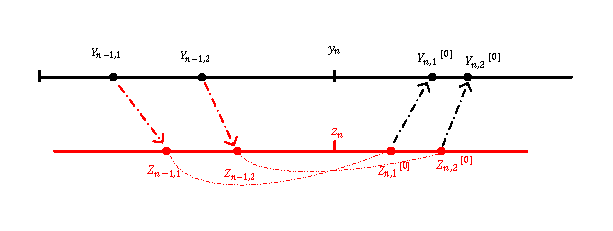
\includegraphics[width=12cm, height=6cm] {AtalenHasieraketa3}}
\caption[Atalen hasieraketa (Kepler fluxuaren aldagai aldaketa)]{\small Atalen hasieraketarako, Kepler fluxuan oinarritutako aldagai aldaketaren aplikazioa}
\label{fig:aldflx}
\end{figure} 

Ohiko polinomio interpolatzailearen bidez hasieraketa ona izateko, urratsa txikia izan behar du. Teknika hau erabiliz, interpolazioaren errorea $\mathcal{O}(\epsilon)$ mailakoa izango da eta urratsa handia erabili arren, hasieraketa ona izango dugu.


\section{Paralelizazioa.}


Hasierako baliodun problemen,
\begin{equation}
 \label{eq:eztivp}
\dot{y}(t)=f(t,y(t)), \ f: \mathbb{R}^{d+1} \longrightarrow \mathbb{R}^d, \ \ y(t_0)=y_0,
\end{equation} 
integrazioetan, denboran zehar zenbakizko soluzioa sekuentzialki lortzen goaz eta beraz, ez dago  paralelizazioa modu zuzenean aplikatzerik. Hala ere, hainbat teknika proposatu dira \cite{Burrage1993}, eta etorkizunean paralelizazio garapen berriak espero dira.   

Saha eta Tremainek \cite{Saha1996}, eguzki-sistemaren epe luzeko integrazioetarako, metodo paraleloa proposatu zuten. Konputazio paraleloa lortzeko, integrazio tarteen (1-astea, 2-astea,\dots) integrazioak prozesadoreen artean banatzen dituzte. Ondoren, teknika hau garatuz, Laskar-ek \cite{Jimenez-Perez2011} bere proposamen berria egin zuen. Hairer-ek \cite{Gander2014}, Hamiltondar sistemetan inplementazio hauen  analisia egin zuen eta aplikatzeko, hainbat eragozpen zeudela ondorioztatu zuen.

Ebatzi nahi den problemaren ekuazio diferentzialen balioztapena, konputazionalki garestia bada edota dimentsio handikoa, paralelizazioa beste maila batean aplika daiteke. Paralelizazioa aplikatzeko bide bat, dimentsio handiko ekuazio-sistemaren balioztapena, osagai independentetan banatzea eta hauen konputazioa, prozesadore batzuen artean modu paraleloan kalkulatzea da. Problema zurruna denean, metodo inplizituak aplikatzen direnez, urrats bakoitzean, dimentsio handiko ekuazio-sistemak ebatzi behar dira eta horretarako, paralelizazioan oinarritutako inplementazio (\emph{LAPACK}) eraginkorrak ditugu. Era berean, N-gorputzeko problemetan, $N$ handia denean, gorputzen arteko interakzioak ($\mathcal{O}(N^2)$) kalkulatzeko         
paralelizazioan oinarritutako hainbat inplementazio \cite{Barnes1986,Carrier1988,Driscoll2013} aplika daitezke. 

IRK metodoei dagokienez, $f(Y_i), \ i=1,\dots,s$ ataletako funtzio balioztapena paraleloan exekuta daiteke. Eguzki-sistemaren eredu errealistetan, $f$ funtzioa konplexua izango da eta beraz, paralelizazioa aplikatzeak abantaila izango du. Bestalde, doitasun bikoitzeko integrazioetarako, Gauss metodoaren inplementazio estandar eraginkorrena, $s=6$ atalekoa kontsideratzen da \cite{Hairer2006}. Eguzki-sistemaren integraziorako gure inplementazioa, ordea, $s=8$ ataletako metodoa eraginkorra da eta honek, paralelizioak abantaila handiago suposatzen du.    


\section{Inplementazioaren erabilgarritasuna.}


Inplementazioa, eguzki-sistemaren doitasun altuko epe luzeko integrazioetan aplikatzeaz gain, beste N-gorputzeko problema batzuetan aplikatzea eraginkorra izan daitekeen hausnartuko dugu. 

\subsection*{Efemerideak.}

Eguzki-sistemaren  efemerideek, eguzki-sistemaren eredu konplexuak eta epe tarte txikietarako (ehunka urtekoak) integrazioak konputatzen dituzte. Konputagailuen erabilera hasi aurretik, efemerideak teoria analitikoetan oinarritutako serie funtzioen bidez kalkulatzen ziren. Soluzio hauetan, Fourier-en serie trigonometriko luzeen ebaluazioa egin behar zen. $1960.$ hamarkadan, eguzki-sistemaren ezagutza hobetu zenean (espazio bidaiak eta behatoki astronomikoen aurrerapenak medio), serie oso luzeak kalkulatu behar zituzten, eta orduan zenbakizko integrazioen metodoak, eraginkorragoak bilakatu ziren \cite{Kaplan2015}.   
   
Eguzki-sistemaren gorputzen efemeride modernoak, aldaketa adierazten duten (\ref{eq:nbody})  ekuazio diferentzialen  zenbakizko integrazioaren bidez kalkulatzen dira. Integrazioaren hasierako balioak eta ereduaren parametroak, sateliteen bidez jasotako datuekin alderatzen dira.

Efemerideen soluzioak \emph{Chebyshev} polinomio moduan adierazten dira. Zenbakizko integrazio hauetan, biribiltze errorea gai garrantzitsua da. $128$-biteko aritmetikaren aukera baztertzen da, konputazioa oso garestia delako eta $64$-biteko doitasuneko aritmetika hobetzen dituzten  konputazionalki teknika merkeak, aplikatzen dira. 

Efemerideetarako, eguzki-sistemaren eredu konplexua aplikatzen da. Gorputz nagusien arteko indar grabitazionalez gain, erlatibitate efektua, asteroideek eragindako grabitazio indarrak, gorputzen formen eragina eta beste hainbat indar ez grabitazionalak kontutan hartzen dituzte. Mugimenduaren ekuazio diferentzialak, era honetakoak izaten dira \cite{Feinga2015},      
      \begin{equation*}
      \ddot{x}_{Planet}= \sum_{A \neq B} \mu_B \frac{r_{AB}}{\|r_{AB}\|^3}+\ddot{x}_{GR} (\beta,\gamma,c^{-4})+ \ddot{x}_{AST,300}+ \ddot{x}_{J_2}.
      \end{equation*}

Hauek dira, ekuazio hauen konplexutasuna erakusten duten ezaugarri batzuk:      
      \begin{itemize}
      \item Gorputz kopurua: $8$ planetak, Ilargia, Pluton eta 300 asteroide. Asteroideek, bereziki Marte planetaren mugimenduarengan dute eragina (\ref{fig:asteroideak} irudia) eta kontutan hartzekoak dira, barne-planeten mugimenduaren doitasun handiko emaitzak behar ditugunean . Bost asteroide nagusiren masak (Ceres, Pallas, Vesta, Iris eta Bamberga) Merkurio eta Pluton planeten mailakoak direnez, integrazioetan gehitzen dira. Gainontzeko asteroide txikien talde handiak, estimazioen bidez simulatzen dira.
      \item Erlatibitate efektua (GR): Einstein-Imfeld-Hoffmann, $c^{-4}$ PPN hurbilketa.
      \item $J_2$: eguzkia esferikoa ez izatearen eragina. 
      \item Integrazioaren urrats luzera, $h=0.055$ egunekoa da.
      \end{itemize}   


\begin{figure} [h]
\centerline{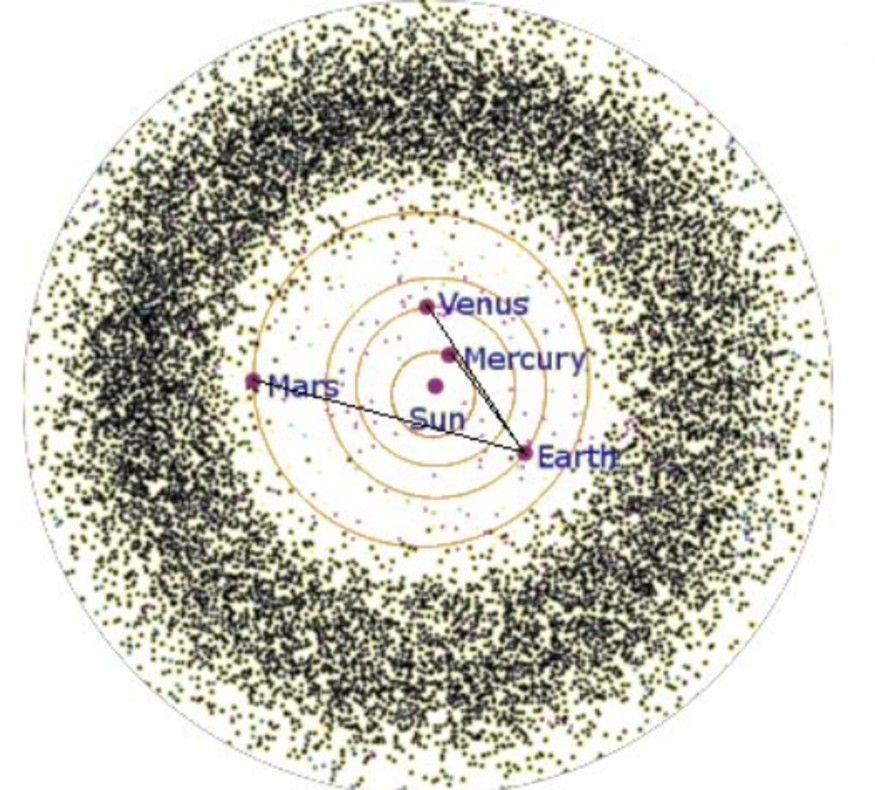
\includegraphics [width=6cm, height=5cm] {Asteroideak}}
\caption[Asteroideak]{\small Marte eta Jupiter planeten artean kokatzen dira asteroide kopuru handi bat.}
\label{fig:asteroideak}
\end{figure} 

  
\subsubsection*{Hiru efemerideak.}

Gaur-egun, eguzki-sistemaren planeten hiru efemeride kalkulatzen dira.
\begin{enumerate}
\item Jet Propulsion Laboratory (\emph{EEBB}) \emph{NASA}-ko erakundeak DE (Development Ephemerides) izeneko efemerideak konputatzen ditu.

      $1984$.urtean kalkulatu zen lehen efemeridea (DE-200) eta $2.014$.urteko \emph{DE-430} \cite{Folkner2014} efemeridea publikatutako azkena da. Azken efemeride honen integrazio tartea, $1550-2650$ artekoa izan da.

      Zenbakizko integrazio metodoa, urrats luzera eta  ordena aldakorreko \emph{Multistep Adams} metodoa \cite{Krogh1997} (\emph{DIVA}/\emph{QIVA}) da. \emph{QIVA} doitasun laukoitzeko ($128$-bit) bertsioari deitzen zaio: mugimenduaren ekuazioen Newton zatia, doitasun laukoitzean kalkulatzen da eta ekuazioaren gainontzeko zatia, doitasun bikoitzean.

\item Institut de Méchanique Céleste et de Calcul des Ephémérides (IMCCE, Paris Observatory) INPOP (Intégrateur Númerique Planétaire de l'Observatoire de Paris) izeneko efemerideak.
      
      $2.000$.urteraino, efemerideen kalkulua teori analitikoetan oinarritzen zituzten. $2.003$.urtean, zenbakizko integrazioaren bidezko lehen efemeridea kalkulatu zuten eta \emph{INPOP13c} efemeridea \cite[$2.014$]{Fienga2008} publikatutako azkena da.
           
	  Zenbakizko integrazio metodoa: $12$ ordenako \emph{Adams-Cowell} metodoa da eta urrats finkoa aplikatzen dute.
	  
	  Doitasuna: C lengoaian inplementatuta dago eta \emph{Intel} makinetako $80$-biteko doitasuna erabiltzen du \cite{Fienga2008}.  
	  
  
\item Institute of Applied Astronomy (\emph{IAA}, St. Petersburg), EPM (Ephemerides Planets-Moon) izeneko efemerideak.
      
      $1.980$.urtetik aurrera, zenbakizko integrazioen bidezko efemerideak kalkulatu dituzte eta  \emph{EPM2013} efemeridea \cite[2.014]{Pitjeva2014} publikatutako azkena  da.
      
      Zenbakizko integrazio metodoa, \emph{Everhart} izeneko \emph{IRK} metodoa (Gauss-Radau) da. $23$ ordenako metodoa eta urrats luzera finkoa aplikatzen dute.
            
      Doitasuna. Inplementazioak (ERA izeneko softwarea), \emph{Intel} makinetako $80$-biteko doitasuna erabiltzen du.
      
\end{enumerate}

\subsection*{Satelite artifizialen problemak.}
    
Satelite artifizialen problemak, gure inplementazioaren erabilgarritasunaren adibide argiak dira. Problema hauetan, eredu matematiko konplexuak erabiltzen dira, konputazionalki garestiak, eta sateliteen kokapenaren eboluzioa, zehaztasun handiarekin ezagutu behar da. Ondorioz, integrazio metodo eraginkorrak eta  ordena altuko metodoak aplikatu behar dira \cite{Beylkin2014}.    

\subsection*{Exoplanetak.}

Eguzki-sistemari egokitutako splitting metodo sinplektikoak \cite{Wisdom1991,Laskar2001}, eguzki-sistemaren problemaren bi ezaugarriei abantaila atereaz diseinatzen dira. Lehenik, planeten eguzkiarekiko orbitak ia Kepleriarrak dira. Bigarrenik, N-gorputzen problemaren formulazio Hamiltondarrean oinarritzen dira eta sinplektikoak direnez, Hamiltondarra zehazki mantentzen dute. 

Exoplaneta sistemak integratzeko metodo berriak behar dira \cite{Fabrycky2010}. Exoplaneten planeta-sistemen mugimenduak ez dira eguzki-sistemarenak bezain egonkorrak. Exoplaneta sistemetan, eszentrikotasun handiko orbitak, periodo txikikoak, eta izar anitzeko planeta-sistemak aurkituko ditugu. Splitting metodo sinplektikoak, ez dira ondo egokitzen era honetako sistemak integratzeko.
IRK Gauss metodoa, edozein sistema integratzeko aplika daiteke. Eguzki-sistemaren ekuazioei aldagai aldaketa modu egokian aplikatuz, metodoa lehiakorra da eta exoplaneta-sistemak integratzeko ere,  baliagarria izan daitekeela pentsatzen dugu. Dena den, exoplaneta sistemen datuen doitasuna txikia da  eta beraz, ez du zentzu handirik doitasun handiko integrazioak egitea.         
 
\subsection*{Molekulen sistema dinamikoak.}

Molekulen dinamikaren problema, Hamiltondarra da eta ekuazio diferentzialak era honetan idatzi daitezke,
\begin{align*}
&\dot{q}_i=v_i, \\
&\dot{v}_i=g(q_i), \ i=1,\dots,N,
\end{align*}
non $N$ partikulen kopurua eta $q_i,v_i \in \mathbb{R}^3$ diren.

Molekulen sistema dinamikoen integrazioak konputazionalki garestiak dira, $N$ balioa handia delako, $g$ funtzioaren konplexutasunagatik eta integrazioa epea luzea izaten delako. Molekulen sistema dinamikoen integrazioetarako, \emph{Störmer-Verlet} (\ref{eq:stverlet}) metodo erabilienetakoa da. Sanz Sernak \cite{sserna1996}, molekulen sistema dinamikoen integraziorako Gauss metodoen eraginkortasuna aztertu zuen, eta \emph{Störmer-Verlet} metodoa eraginkorragoa zela ondorioztatu zuen.
Molekulen sistema dinamikoen integrazioetarako gure planteamenduak, ez da argia aplikatu daitekeenik. 



